% Chapter 4, Topic _Linear Algebra_ Jim Hefferon
%  http://joshua.smcvt.edu/linearalgebra
%  2001-Jun-12
\topic{Kecepatan Menghitung Determinan}
Bagi matriks besar, mencari determinan dengan operasi baris biasanya jauh lebih
cepat daripada menggunakan ekspansi permutasi.
Kita akan memperjelas pernyataan ini dengan menentukan banyak operasi yang
dijalankan oleh setiap metode.

Untuk membandingkan kecepatan dua algoritma, bagi masing-masing algoritma kita
menentukan bagaimana waktu yang diperlukan bertumbuh ketika ukuran himpunan data
masukannya bertambah.
Sebagai contoh, jika ukuran masukan diperbesar dengan faktor sepuluh, apakah
waktu yang diperlukan bertambah dengan faktor sepuluh, seratus, atau seribu?
Artinya, apakah waktu yang diperlukan sebanding dengan ukuran himpunan data,
kuadrat ukurannya, kubik ukurannya, dan seterusnya?
Algoritma yang waktunya sebanding dengan kuadrat lebih cepat daripada algoritma
yang waktunya sebanding dengan kubik.

Pertama-tama, tinjau rumus ekspansi
permutasi.\index{determinan!ekspansi permutasi}%
\index{ekspansi permutasi}
\begin{equation*}
   \begin{vmat}
      t_{1,1}  &t_{1,2}  &\ldots  &t_{1,n}  \\
      t_{2,1}  &t_{2,2}  &\ldots  &t_{2,n}  \\
               &\vdots                      \\
      t_{n,1}  &t_{n,2}  &\ldots  &t_{n,n}
   \end{vmat}
   =\!\!\sum_{\text{permutasi\ }\phi}\!\!\!\!
     t_{1,\phi(1)}t_{2,\phi(2)}\cdots t_{n,\phi(n)}
                                 \deter{P_{\phi}}   
   % &=
   % \begin{aligned}[t]
   %    &t_{1,\phi_1(1)}\cdot t_{2,\phi_1(2)}\cdots
   %         t_{n,\phi_1(n)}\deter{P_{\phi_1}}       \\  %[.25ex]
   %    &\hbox{}\quad\hbox{}
   %      +t_{1,\phi_2(1)}\cdot t_{2,\phi_2(2)}\cdots
   %         t_{n,\phi_2(n)}\deter{P_{\phi_2}}       \\
   %    &\hbox{}\quad\hbox{}\vdotswithin{+}             \\
   %    &\hbox{}\quad\hbox{}
   %      +t_{1,\phi_k(1)}\cdot t_{2,\phi_k(2)}\cdots
   %         t_{n,\phi_k(n)}\deter{P_{\phi_k}} 
   % \end{aligned}
\end{equation*}
Terdapat $n!=n\cdot(n-1)\cdots 2\cdot 1$ permutasi atas $n$ unsur yang berbeda.
Karena itu, bagi matriks dengan $n$~baris, jumlah ini memiliki $n!$ suku.
Pembentukan hasil kali $n$ entri pada setiap suku memerlukan $n-1$ perkalian,
disertai kemungkinan perubahan tanda oleh $\deter{P_\phi}$.
Fungsi faktorial bertumbuh cepat:~bahkan ketika $n$ hanya $10$, ekspansi tersebut
sudah memiliki $10!=3\,628\,800$ suku.
Perhatikan bahwa pertumbuhan yang sebanding dengan faktorial lebih besar daripada
pertumbuhan yang sebanding dengan kuadrat, $n!>n^2$ untuk $n$ yang cukup besar.
Perkalian dua faktor pertama dalam $n!$ memberikan $n\cdot(n-1)$, yang untuk $n$
besar kira-kira $n^2$, lalu perkalian dengan faktor-faktor tambahan membuat
faktorial semakin besar. Demikian pula, fungsi faktorial bertumbuh lebih cepat
daripada~$n^3$, dan seterusnya.
Jadi, algoritma yang menggunakan rumus ekspansi permutasi, dan karena itu
menjalankan sekurang-kurangnya sebesar faktorial dari banyaknya baris, akan
sangat lambat.

Sebaliknya, waktu yang diperlukan metode reduksi baris tidak bertumbuh secepat itu.
% Below is a fragment of row-reduction code.
% It is 
% in the computer language \textsc{FORTRAN}, 
% which is widely used for numeric code.
% % (there are no rows below
% % the \lstinline[style=inline]!N!-th 
% % so it is not included in the loop).
% \begin{lstlisting}
% DO 10 ROW=1, N-1
%   PIVINV=1.0/A(ROW,ROW)
%   DO 20 I=ROW+1, N
%     DO 30 J=I, N
%       A(I,J)=A(I,J)-PIVINV*A(ROW,J)
%     30 CONTINUE
%   20 CONTINUE
% 10 CONTINUE
% \end{lstlisting} 
Di bawah ini terdapat skrip reduksi baris dalam bahasa komputer Python.
(\textit{Catatan:}
Kode ini masih naif; misalnya, kode tidak menangani kasus ketika entri
\lstinline[style=inline]!m[p_row][p_row]! bernilai nol.
Analisis versi lengkap yang memuat semua pengujian dan subkasus lebih rumit,
tetapi akan memberikan hasil kecepatan yang kira-kira sama.)
\begin{lstlisting}
import random

def random_matrix(num_rows, num_cols):
    m = []
    for row in range(num_rows):
        new_row = []
        for col in range(num_cols):
            new_row.append(random.uniform(0,100))
        m.append(new_row)
    return m

def gauss_method(m):
    """Jalankan Metode Gauss pada m. Kode ini hanya untuk ilustrasi
    dan tidak boleh digunakan dalam praktik.
      m  daftar yang berisi daftar bilangan; setiap daftar merupakan satu baris
    """
    num_rows, num_cols = len(m), len(m[0])
    for p_row in range(num_rows):
        for row in range(p_row+1, num_rows):
            factor = -m[row][p_row] / float(m[p_row][p_row])
            new_row = []
            for col_num in range(num_cols): 
                p_entry, entry = m[p_row][col_num], m[row][col_num]
                new_row.append(entry+factor*p_entry)
            m[row] = new_row
    return m

response = input('banyak baris? ')
num_rows = int(response)
m = random_matrix(num_rows, num_rows)
for row in m:
    print(row)
M = gauss_method(m)
print("-----")
for row in M:
    print(row)
\end{lstlisting}
Selain rutin untuk menjalankan Metode Gauss, program ini juga memiliki rutin
untuk menghasilkan matriks yang diisi bilangan acak (bilangannya berada antara
$0$ dan~$100$ agar mudah dibaca di bawah).
Program ini meminta banyak baris dari pengguna, menghasilkan matriks persegi
acak dengan ukuran tersebut, lalu menjalankan reduksi baris padanya.
\begin{lstlisting}
$ python gauss_method.py
banyak baris? 4
[69.48033741746909, 32.393754742132586, 91.35245787350696, 87.04557918402462]
[98.64189032145111, 28.58228108715638, 72.32273998878178, 26.310252241189257]
[85.22896214660841, 39.93894635139987, 4.061683241757219, 70.5925099861901]
[24.06322759315518, 26.699175587284373, 37.398583921673314, 87.42617087562161]
-----
[69.48033741746909, 32.393754742132586, 91.35245787350696, 87.04557918402462]
[0.0, -17.40743803545155, -57.37120602662462, -97.2691774792963]
[0.0, 0.0, -108.66513774392809, -37.31586824349682]
[0.0, 0.0, 0.0, -13.678536859817994]
\end{lstlisting}  %$

Di dalam rutin \lstinline[style=inline]!gauss_method!, bagi setiap baris
\lstinline[style=inline]!p_row!, rutin menjalankan
$\text{\lstinline[style=inline]!factor!}\cdot\rho_{\text{\lstinline[style=inline]!p_row!}}+\rho_{\text{\lstinline[style=inline]!row!}}$
pada baris-baris di bawahnya.
Bagi setiap baris di bawah tersebut, operasi ini melibatkan setiap entri pada
baris itu. Jadi, terdapat tiga kalang bertingkat.
Karena itu, waktu jalan program ini kira-kira sebanding dengan kubik banyak
baris dalam matriks.
(\textit{Catatan.}
Kita mengabaikan banyak persoalan. Sebagai contoh, kita mungkin khawatir bahwa
waktu program didominasi oleh waktu untuk menyimpan dan mengambil entri dari
memori, bukan oleh operasi baris. Namun, pengembangan model komputasi berada di
luar cakupan kita.)

Jika kita menambahkan kode berikut di bagian bawah,
\begin{lstlisting}
def do_matrix(num_rows):
    gauss_method(random_matrix(num_rows, num_rows))

import timeit
for num_rows in [10,20,30,40,50,60,70,80,90,100]:
    s = "do_matrix("+str(num_rows)+")"
    t = timeit.timeit(stmt=s, setup="from __main__ import do_matrix",
                      number=100)
    print("banyak_baris=", num_rows, " detik=", t)
\end{lstlisting}
maka Python akan mengukur waktu program.
Berikut adalah keluaran dari satu eksekusi yang diukur waktunya.
\begin{lstlisting}
banyak_baris= 10  detik= 0.0162539482117
banyak_baris= 20  detik= 0.0808238983154
banyak_baris= 30  detik= 0.248152971268
banyak_baris= 40  detik= 0.555531978607
banyak_baris= 50  detik= 1.05453586578
banyak_baris= 60  detik= 1.77881097794
banyak_baris= 70  detik= 2.75969099998
banyak_baris= 80  detik= 4.10647988319
banyak_baris= 90  detik= 5.81125879288
banyak_baris= 100  detik= 7.86893582344  
\end{lstlisting}
Menggambarkan data tersebut menghasilkan sebagian kurva kubik.
\begin{center}
  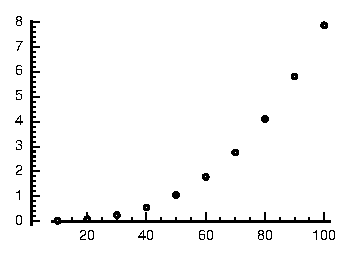
\includegraphics{det/bin/detspeed.pdf}
\end{center}

Menemukan algoritma tercepat untuk menghitung determinan merupakan topik riset
yang masih aktif. Sejauh ini, peneliti telah menemukan algoritma dengan waktu
jalan di antara kuadrat dan kubik banyak baris.

Perbedaan waktu antara kedua metode perhitungan determinan, yaitu ekspansi
permutasi dan operasi baris, menunjukkan bahwa meskipun secara prinsip keduanya
memberikan jawaban yang sama, dalam praktik kita menginginkan metode dengan
kinerja terbaik.


\begin{exercises}
  % \item[\textit{Most of these presume access to a computer.}]
  \item 
    Untuk memperoleh gambaran tentang perilaku matriks biasa, kita dapat
    memanfaatkan kemampuan sistem komputer menghasilkan bilangan acak (tentu
    saja, bilangan ini hanya acak semu karena berasal dari algoritma, tetapi
    bilangan tersebut lolos sejumlah uji statistik yang wajar bagi keacakan).
    \begin{exparts}
      \partsitem Isi larik $\nbyn{5}$ dengan bilangan acak, misalnya dalam
        rentang $\clopinterval{0}{1}$.
        Periksa apakah larik itu singular. Ulangi percobaan beberapa kali.
        Dalam pengertian ini, apakah matriks singular sering atau jarang muncul?
      \partsitem Ukur waktu yang diperlukan sistem aljabar komputer Anda untuk
        mencari determinan sepuluh larik bilangan acak berukuran $\nbyn{10}$.
        Temukan waktu rata-rata per larik.
        Ulangi butir sebelumnya bagi larik $\nbyn{20}$, $\nbyn{30}$, \ldots,
        $\nbyn{100}$, lalu bandingkan dengan bilangan di atas.
        (Perhatikan bahwa ketika suatu larik singular, kadang-kadang kita dapat
        menentukan dengan cepat bahwa matriks tersebut singular, misalnya jika
        baris pertama sama dengan baris kedua. Berdasarkan jawaban Anda pada
        bagian pertama, apakah Anda mengharapkan matriks singular berperan besar
        dalam rata-rata tersebut?)
      \partsitem Gambarkan ukuran masukan terhadap waktu rata-rata.
    \end{exparts}
    \begin{answer}
      Hasil pengukuran waktu sebagian bergantung pada sistem aljabar komputer
      yang Anda gunakan dan sebagian pada kemampuan komputer tempat perhitungan
      dijalankan. Namun, Anda seharusnya memperoleh kurva yang serupa dengan
      kurva yang ditampilkan.
%       \begin{exparts}
%         \partsitem Under Octave, \texttt{rank(rand(5))} finds the
%           rank of a $\nbyn{5}$ matrix whose entries are (uniformly
%           distributed) in the interval $[0..1)$.
%           This loop which runs the test $5000$ times
% \begin{lstlisting}
% octave:1> for i=1:5000
% > if rank(rand(5))<5 printf("That's one."); endif
% > endfor
% \end{lstlisting}  
%           produces (after a few seconds) returns the prompt, with no output.

%           The Octave script
% \begin{lstlisting}
% function elapsed_time = detspeed (size)
%   a=rand(size);
%   tic();
%   for i=1:10
%      det(a);
%   endfor
%   elapsed_time=toc();
% endfunction
% \end{lstlisting}  
%           lead to this session (obviously, your times will vary). 
% \begin{lstlisting}
% octave:1> detspeed(5)
% ans = 0.019505
% octave:2> detspeed(15)
% ans = 0.0054691
% octave:3> detspeed(25)
% ans = 0.0097431
% octave:4> detspeed(35)
% ans = 0.017398
% \end{lstlisting}  
%           \partsitem Here is the data (rounded a bit), and the graph.
%             \begin{center}
%               \begin{tabular}{l}
%               \begin{tabular}{r|cccccc}
%                  \textit{matrix rows} 
%                     &$15$ &$25$ &$35$ &$45$ &$55$ &$65$  \\
%                  \hline
%                  \textit{time per ten}
%                     &$0.003\,4$                     
%                     &$0.009\,8$
%                     &$0.067\,5$
%                     &$0.028\,5$ 
%                     &$0.044\,3$
%                     &$0.066\,3$ 
%               \end{tabular}                                       \\
%               \qquad\begin{tabular}{r|ccc}
%                  \textit{matrix rows} 
%                     &$75$ &$85$ &$95$ \\
%                  \hline
%                  \textit{time per ten}
%                     &$0.142\,8$  
%                     &$0.228\,2$ 
%                     &$0.168\,6$              
%               \end{tabular}
%               \end{tabular}
%             \end{center}
%           This data is from an average of twenty runs of the above script,
%           because of the possibility that the randomly chosen matrix
%           happens to take an unusually long or short time.
%           Even so, the timing cannot be relied on too heavily; this is
%           just an experiment.
%           \begin{center}
%             \includegraphics[width=0.4\textwidth]{det/mp/ch4.28}
%           \end{center}
%       \end{exparts}
    \end{answer}
  \item 
    Hitung determinan masing-masing matriks berikut dengan tangan menggunakan
    kedua metode yang dibahas di atas.
    \begin{exparts*}
      \partsitem $\begin{vmat}[r]
                    2  &1  \\
                    5  &-3
                  \end{vmat}$
      \partsitem $\begin{vmat}[r]
                    3  &1  &1  \\
                   -1  &0  &5  \\
                   -1  &2  &-2 
                  \end{vmat}$
      \partsitem $\begin{vmat}[r]
                    2  &1  &0  &0  \\
                    1  &3  &2  &0  \\
                    0  &-1 &-2 &1  \\
                    0  &0  &-2 &1
                  \end{vmat}$
    \end{exparts*}
    Hitung banyak perkalian dan pembagian yang digunakan dalam setiap kasus bagi
    masing-masing metode.
    % (Computer multiplications and divisions take 
    %  longer than additions and subtractions, so algorithm 
    %  designers worry about them more.)
     \begin{answer}
       Banyak operasi bergantung pada cara persis kita menjalankannya.
       \begin{exparts}
         \partsitem Determinannya adalah $-11$.
           Reduksi baris memerlukan satu kombinasi baris dengan satu pembagian
           untuk membentuk faktor $-5/2$ dan dua perkalian
           ($-5/2$ kali $2$ ditambah $5$, serta $-5/2$ kali $1$ ditambah $-3$).
           Hasil kali sepanjang diagonal memerlukan satu perkalian lagi.
           Ekspansi permutasi memerlukan dua perkalian ($2$ kali $-3$ dan $5$
           kali $1$).
         \partsitem Determinannya adalah $-39$.
           Jika setiap operasi baris hanya memperbarui bagian baris yang masih
           aktif, reduksi menggunakan tiga pembagian, delapan perkalian dalam
           operasi baris, dan dua perkalian pada diagonal, jadi totalnya tiga
           belas perkalian atau pembagian.
           Ekspansi permutasi memiliki enam suku, masing-masing dengan dua
           perkalian, jadi menggunakan dua belas perkalian.
         \partsitem Determinannya adalah $4$.
           Dengan konvensi yang sama, tiga operasi eliminasi menggunakan tiga
           pembagian dan sembilan perkalian, lalu hasil kali diagonal memakai
           tiga perkalian lagi, jadi totalnya lima belas perkalian atau
           pembagian.
           Ekspansi penuh memiliki $4!=24$ suku dengan tiga perkalian per suku,
           jadi menggunakan tujuh puluh dua perkalian sebelum memanfaatkan
           entri-entri nol.
       \end{exparts}
     \end{answer}
  \item Penggunaan \lstinline[style=inline]!do_matrix! oleh rutin pengukur waktu
    memiliki kekeliruan.
    Rutin tersebut menjalankan dua hal, yaitu menghasilkan matriks acak lalu
    menjalankan \lstinline[style=inline]!gauss_method! padanya, sehingga waktu
    yang dikembalikan berlaku bagi gabungan keduanya.
    Buat kode yang hanya mengukur waktu rutin
    \lstinline[style=inline]!gauss_method!.
    \begin{answer}
      Bangun terlebih dahulu kumpulan matriks masukan, lalu ukur hanya reduksinya.
      Perhatikan bahwa \lstinline[style=inline]!gauss_method! seperti ditulis di
      atas mengubah matriks masukan. Karena itu, setiap pengulangan harus memakai
      salinan baru dari matriks awal; jika tidak, semua pengulangan setelah yang
      pertama bekerja pada matriks berbentuk eselon. Waktu penyalinan juga harus
      dikeluarkan dari pengukuran jika yang ingin diukur hanya reduksinya.
      Sebagai contoh, siapkan seratus matriks terlebih dahulu, lalu ukur setiap
      reduksi tepat satu kali.
\begin{lstlisting}
matrices = [random_matrix(num_rows, num_rows) for _ in range(100)]
t = timeit.timeit(
        stmt="for m in matrices: gauss_method(m)",
        setup="from __main__ import gauss_method, matrices",
        number=1)
\end{lstlisting}
    \end{answer}
  \item 
    Larik $\nbyn{10}$ apa yang dapat Anda rancang agar paling lama direduksi oleh
    komputer Anda? Larik apa yang paling cepat?
    \begin{answer}
      Bagi implementasi yang ditampilkan di atas, setiap masukan $\nbyn{10}$ yang
      berhasil diselesaikan menjalankan tepat $45$ pembagian faktor, $450$
      perkalian entri, dan $450$ penjumlahan. Karena kalangnya tidak melewati
      operasi yang tidak perlu, matriks identitas tidak lebih cepat daripada
      matriks padat; struktur matriks hanya dapat mengubah hasil dengan
      menyebabkan kegagalan pivot nol.
      Implementasi yang dioptimalkan dapat memanfaatkan struktur khusus.
      Dalam sistem aljabar eksak, bilangan bulat dengan banyak digit juga dapat
      memperlambat aritmetika meskipun banyak operasinya sama.
      (Sebagian sistem aljabar komputer juga dapat menghasilkan matriks khusus;
      cobalah beberapa di antaranya.)
      % One way to get started is to compare these under Octave:
      % \texttt{det(rand(10));}, versus
      % \texttt{det(hilb(10));}, versus
      % \texttt{det(eye(10));}, versus
      % \texttt{det(zeroes(10));}. 
      % You can time them as in \texttt{tic(); det(rand(10)); toc()}.
    \end{answer}
%   \item 
%     Write the rest of the FORTRAN program to do a
%     straightforward implementation of calculating determinants via
%     Gauss's Method.
%     (Don't test for a zero leading entry.)
%     Compare the speed of your code to that used in your computer algebra
%     system.
%     \begin{answer}
%       This is a simple one.
% \begin{lstlisting}
% DO 5 ROW=1, N
%    PIVINV=1.0/A(ROW,ROW)
%    DO 10 I=ROW+1, N
%       DO 20 J=I, N
%          A(I,J)=A(I,J)-PIVINV*A(ROW,J)
%       20 CONTINUE
%    10 CONTINUE
% 5 CONTINUE
% \end{lstlisting}     
%     \end{answer}
  \item Sebagian spesifikasi bahasa komputer mengharuskan larik disimpan
    ``menurut kolom'', yaitu seluruh kolom pertama disimpan bersebelahan,
    kemudian kolom kedua, dan seterusnya.
    Apakah fragmen kode yang diberikan memanfaatkan hal ini, atau dapatkah kode
    tersebut ditulis ulang agar lebih cepat dengan memanfaatkan fakta bahwa
    pengambilan data oleh komputer lebih cepat dari lokasi yang bersebelahan?
    \begin{answer}
      Tidak. Kode di atas menangani bilangan menurut baris.
    \end{answer}
\end{exercises}
\endinput
